\section{Selección de características}

En \cite{9137899} combinan técnicas simples de eliminación de ruido, distribución desequilibrada de clases y selección de métricas de software para optimizar la predicción de defectos en software. La técnica fue probada en diez conjuntos de datos de predicción de fallos de software. Los resultados experimentales, incluyendo la recall, precisión, medida-F, exactitud y los valores de ROC-AUC, muestran que el método propuesto mejora el rendimiento de la predicción de fallos y los resultados obtenidos son mejores o cercanos a varios modelos comparativos. Se utilizan los conjuntos de datos NASA, Promise, y Github, combinando con los clasificadores: regresión logística, random forest (RF), SVM, naive Bayes.

\begin{figure}[H]
    \centering
    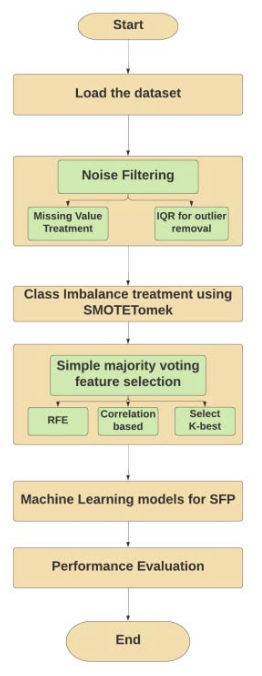
\includegraphics[]{chapters/ChapterMarcoTeorico/sections/FeaturesSelection/fig/Framework defining Methodology adopted for Software Defect.png}
    \setstretch{1} %Interlineado 1
	\captionsetup{labelsep=period, labelfont=bf}
    \caption{Marco que define la metodología adoptada para la predicción de defectos de software. Tomado desde \cite{9137899}}
    \label{fig:Frameworksd}
\end{figure}

En el paso de Selección de Características por Votación Mayoritaria Simple se utiliza un algoritmo de selección de atributos por votación mayoritaria simple para combinar el resultado de tres técnicas de selección de características, es decir, RFECV (eliminación recursiva de características con validación cruzada), selección de características basada en correlación y la técnica de seleccionar las k mejores.

En \cite{kondo2019impact} se utilizan tres Conjuntos de datos (PROMISE,NASA, AEEEM) sumando 26 proyectos en los que varian las metricas y la cantidad de registros.


\section{Datos Desbalanceados}

En la práctica, los modelos de predicción de defectos de software (SDP) a menudo sufren de datos muy desequilibrados, lo que dificulta a los clasificadores identificar instancias defectuosas. Recientemente, se propusieron muchas técnicas para abordar este problema; la técnica de sobremuestreo es uno de los métodos más conocidos para abordar el problema del desequilibrio de clases. Esta técnica equilibra el número de instancias defectuosas y no defectuosas generando nuevas instancias defectuosas.

Motivados por esto en \cite{8861051}, proponemos un enfoque de Sobremuestreo Basado en Clústeres con Filtrado de Ruido (KMFOS) para abordar el problema del desequilibrio de clases en SDP. KMFOS primero divide las instancias defectuosas en $K$ clústeres, y se generan nuevas instancias defectuosas por interpolación entre instancias de cada dos clústeres. Después de esto, estas nuevas instancias defectuosas se dispersarán diversamente en el espacio del conjunto de datos defectuoso. Luego, extendemos este sobremuestreo basado en clústeres mediante la Identificación de Ruido de Lista Cercana (CLNI) para limpiar las instancias de ruido. Realizamos experimentos extensivos en 24 proyectos para comparar KMFOS con algunos enfoques de sobremuestreo como SMOTE, BorderlineSMOTE, ADASYN, sobremuestreo aleatorio (ROS), SMOTE de K-medias, SMOTE + IPF, SMOTE + ENN y SMOTE + Enlaces de Tomek utilizando cinco clasificadores de predicción.
 

\begin{figure}[H]
    \centering
    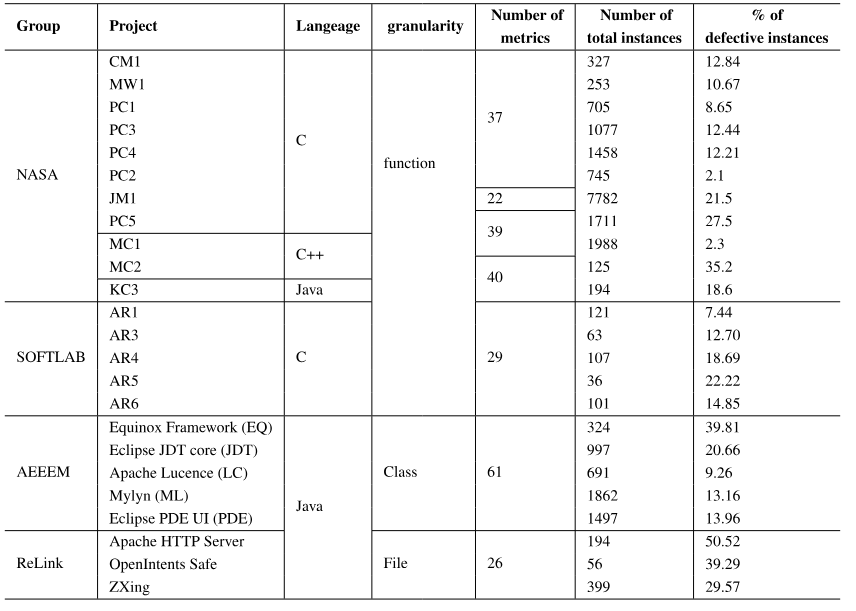
\includegraphics[width=\textwidth]{chapters/ChapterMarcoTeorico/sections/FeaturesSelection/fig/experimental dataset.png}
    \setstretch{1} %Interlineado 1
	\captionsetup{labelsep=period, labelfont=bf}
    \caption{Lista de datasets utilizados. Tomado desde \cite{8861051}}
    \label{fig:desequilibrioDataset}
\end{figure}

De la Figura \ref{fig:desequilibrioDataset}, podemos ver: i) los lenguajes de desarrollo de estos proyectos incluyen Java, C y C++; ii) la granularidad de las métricas cubre función, clase y archivo; iii) el número de instancias varía mucho y la proporción de instancias para la mayoría de los proyectos está muy por debajo del 25\%. Por lo tanto, estos proyectos pueden ser utilizados como objetos experimentales para evaluar estos enfoques con desequilibrio de clases.

En \cite{9044596} se utilizan los proyetos  cm1, kc1, mc2 y pc1 del repositorio PROMISE. Utilizan los clasificadores Logistic regression, NB, Decision tree, MNB y KNN combinados con las tecnicas de remuestreo SMOTE, ROS y RUS.
En la primera fase, aplican las técnicas de remuestreo para todos los clasificadores. En la segunda fase, la combinación de técnica de remuestreo y clasificador que ha tenido mejor desempeño se utiliza en el método de promediación de modelos. Esta combinación sobresaliente se obtiene a partir de las pruebas estadísticas. Su objetivo encontrar el conjunto sobresaliente de clasificador con técnica de remuestreo.



